\documentclass{article}
\usepackage{fontspec}
\usepackage[english]{babel}
\usepackage{tikz}
\usetikzlibrary{shapes.geometric,arrows.meta,positioning}

\begin{document}
\section{TikZ Diagram}

\begin{figure}[h]
\centering
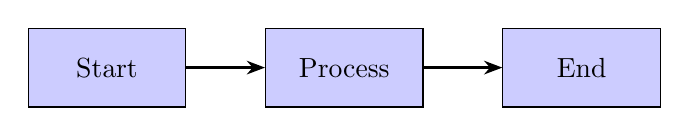
\begin{tikzpicture}[
    box/.style={rectangle, draw, fill=blue!20, minimum width=2cm, minimum height=1cm},
    arrow/.style={->, >=Stealth, thick}
]
\node[box] (A) {Start};
\node[box, right=of A] (B) {Process};
\node[box, right=of B] (C) {End};

\draw[arrow] (A) -- (B);
\draw[arrow] (B) -- (C);
\end{tikzpicture}
\caption{Simple Flowchart}
\end{figure}

\begin{figure}[h]
\centering
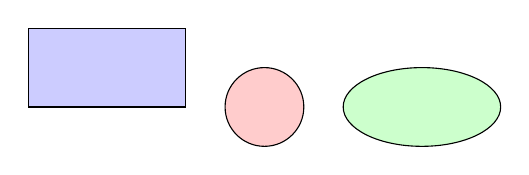
\begin{tikzpicture}
\draw[fill=blue!20] (0,0) rectangle (2,1);
\draw[fill=red!20] (3,0) circle (0.5cm);
\draw[fill=green!20] (5,0) ellipse (1cm and 0.5cm);
\end{tikzpicture}
\caption{Basic Shapes}
\end{figure}
\end{document}
